\head{Запросы суммы и минимума}
Сегодня мы займёмся другими важными линейными алгоритмами, а именно для заданного набора научимся вычислять сумму и минимумы на определённых участках набора (отрезках). Эти алгоритмы часто можно применять в других, более сложных задачах.


\subhead{Запрос суммы}
Первая задача, которую мы разберём будет такая: дан набор $a$ длины $n$, требуется ответить на $q$ запросов сумму на отрезке: $s = a_l + a_{l + 1} + \ldots + a_r$. Называется она \term{RSQ} (range sum query).

Очевидно, как решать эту задачу за \O{n \cdot q} — просто для каждого запроса будем перебирать нужные элементы и искать их сумму. Но ведь понятно, что мы будем часто считать одни и те же суммы, а значит алгоритм можно как-то улучшить, чтобы таких лишних операций не делать.

Для этого воспользуемся идеей предподсчёта. Поэтому нужно придумать, что бы такого посчитать заранее, чтобы потом легко отвечать на запросы. При этом понятно, что подсчитывать мы будем какие-то суммы, остаётся лишь определиться какие именно.\\
\begin{minipage}[c]{0.40\linewidth}
    \setlength{\parindent}{1cm}
    \indent Оказывается, что достаточно подсчитать $p_i$ — сумму первых $i$ элементов: $p_0 = 0,\ p_1 = a_1,\ p_2 = a_1 + a_2,\ \ldots,\ p_n = a_1 + a_2 + \ldots + a_n$. Причём понятно, как вычислить эти числа быстро, это ведь динамика с $p_0 = 0$ и $p_i = p_{i - 1} + a_i$, для $1 \leq i \leq n$.
    
    А теперь нужно понять, зачем мы вообще это посчитали. Для этого попробуем выразить сумму $s$ через элементы $p$: давайте добавим и вычтем первые элементы набора $s = (a_l + a_{l + 1} + \ldots + a_{r}) + (a_1 + a_2 + \ldots + a_{l - 1}) - (a_1 + a_2 + \ldots + a_{l - 1})$. Но ведь теперь мы можем сгруппировать первые две скобки: $s = (a_1 + a_2 + \ldots + a_r) - (a_1 + a_2 + \ldots + a_{l - 1})$, и заметим, что эти скобки — как раз те суммы, которые мы предподсчитали в $p$: $s = p_r - p_{l - 1}$.
\end{minipage}
\begin{minipage}[c]{0.03\linewidth}\ \end{minipage}
\begin{minipage}[c]{0.57\linewidth}
    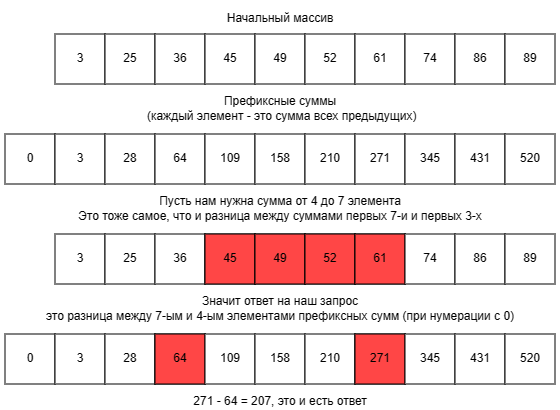
\includegraphics[scale=0.73]{img/prefix_sum.png}
\end{minipage}

Таким образом у нас есть алгоритм, который решает эту задачу: сначала предподсчитаем $p$, а потом будем вычислять ответы для каждого запроса по формуле выше. Так мы за \O{n} сделаем предподсчёт и потом на каждый из $q$ запросов будем отвечать за \O{1}, а значит итоговая сложность — \O{n + q}. Стоит отметить, что вычисленное $p$ называется префиксными-суммами.



\subhead{Двумерные суммы}
Теперь усложним задачу: пусть имеется двумерный набор $a$ из $n$ строк и $m$ столбцов. Требуется для $q$ запросов с параметрами $x_1, y_1, x_2, y_2$ вычислить сумму $s = \sum\limits_{i = x_1}^{x_2} \sum\limits_{j = y_1}^{y_2} a_{i, j}$ (понятно, что $1 \leq x_1 \leq x_2 \leq n$ и $1 \leq y_1 \leq y_2 \leq m$).

Очевидно, что если каждый раз перебирать все элементы, то получим сложность \O{n \cdot m \cdot q}, это, кончено плохо, поэтому можно по одной оси посчитать префикс-суммы, а по другой проходить циклом, и тогда можно получить сложность \O{q \cdot \min(n, m)}. Но понятно, что мы хотим линейный алгоритм, поэтому снова нужно будет что-то предподсчитать, чтобы потом быстро отвечать на каждый из запросов.

Давайте воспользуемся идеей из предыдущей задачи и предподсчитаем $p_{i, j}$ — сумму на прямоугольнике с началом в начале набора $(1, 1)$ и концом в точке $(i, j)$: $p_{i, j} = \sum\limits_{x = 1}^{i} \sum\limits_{y = 1}^{j} a_{x, y}$. Раз у нас есть идея, что предподсчитать, то остаётся лишь две вещи: во-первых, научиться это считать, а во-вторых, использовать это для решения нашей задачи.

Начнём с вычисления $p_{i, j}$. Начало нашей динамики очевидно: $p_{0, 0} = 0$, так как это пустой набор по обеим осям, а также $p_{0, j} = 0$ и $p_{i, 0} = 0$, так как у это тоже пустые наборы, ведь они пусты по одной оси. Теперь поймём, как посчитать $p_{i, j}$, если мы уже знаем $p_{x, y}$, где $x < i$ или $y < j$ (или выполняются оба условия). Во-первых, понятно, что у этой сумме будут $a_{i, j}$, а также соседние числа $a_{i - 1, j}$ и $a_{i, j - 1}$ (если они есть), поэтому давайте попробуем выразить $p_{i, j}$ через ответы для соседей: $p_{i, j} = a_{i, j} + p_{i - 1, j} + p_{i, j - 1} + r$, где $r$ — поправка, чтобы получилась та, сумма  которую мы хотели изначально. Давайте подставим значения для всех слагаемых и выразим $r$: $p_{i, j} = a_{i, j} + \sum\limits_{x = 1}^{i - 1} \sum\limits_{y = 1}^{j} a_{x, y} + \sum\limits_{x = 1}^{i} \sum\limits_{y = 1}^{j - 1} a_{x, y} + r = a_{i, j} + \left( \sum\limits_{x = 1}^{i - 1} \sum\limits_{y = 1}^{j - 1} a_{x, y} + \sum\limits_{x=1}^{i - 1} a_{x, j} \right) + \left( \sum\limits_{x = 1}^{i - 1} \sum\limits_{y = 1}^{j - 1} a_{x, y} + \sum\limits_{y=1}^{j - 1} a_{i, j} \right) + r = \left( a_{i, j} + \sum\limits_{x = 1}^{i - 1} \sum\limits_{y = 1}^{j - 1} a_{x, y} + \sum\limits_{x=1}^{i - 1} a_{x, j} + \sum\limits_{y=1}^{j - 1} a_{i, j} \right) + \left( \sum\limits_{x = 1}^{i - 1} \sum\limits_{y = 1}^{j - 1} a_{x, y} + r \right)$. Теперь остаётся заметить, что первая скобка — как раз требуемая сумма, а значит вторая скобка равна нулю и $r = -\sum\limits_{x = 1}^{i - 1} \sum\limits_{y = 1}^{j - 1} a_{x, y} = -p_{i - 1, j - 1}$. А это значит, что наша формула для подсчёта $p_{i, j}$ будет вот такой:  $p_{i, j} = a_{i, j} + p_{i - 1, j} + p_{i, j - 1} - p_{i - 1, j - 1}$. Также эту формулу можно получить и графически, если закрашивать те элементы, которые мы уже взяли в сумму, то нужно будет вычитать $p_{i - 1, j - 1}$, так как благодаря $p_{i - 1, j}$ и $p_{i, j - 1}$ этот участок покроется дважды, а нужно посчитать его ровно один раз.

Теперь вторая часть — использование наших сумм для ответов на запросы. Для этого заметим, что $p_{x_2, y_2} = \sum\limits_{i = 1}^{x_2} \sum\limits_{j = 1}^{y_2} a_{i, j} = \sum\limits_{i = 1}^{x_1 - 1} \sum\limits_{j = 1}^{y_1 - 1} a_{i, j} + \sum\limits_{i = 1}^{x_1 - 1} \sum\limits_{j = y_1}^{y_2} a_{i, j} + \sum\limits_{i = x_1}^{x_2} \sum\limits_{j = 1}^{y_1 - 1} a_{i, j} + \sum\limits_{i = x_1}^{x_2} \sum\limits_{j = y_1}^{y_2} a_{i, j}$ (мы разбили всю сумму на 4 не пересекающихся области). Теперь добавим и вычтем первое слагаемое ещё раз и перегруппируем слагаемые: $p_{x_2, y_2} = \left( \sum\limits_{i = 1}^{x_1 - 1} \sum\limits_{j = 1}^{y_1 - 1} a_{i, j} + \sum\limits_{i = 1}^{x_1 - 1} \sum\limits_{j = y_1}^{y_2} a_{i, j} \right) + \left( \sum\limits_{i = 1}^{x_1 - 1} \sum\limits_{j = 1}^{y_1 - 1} a_{i, j} + \sum\limits_{i = x_1}^{x_2} \sum\limits_{j = 1}^{y_1 - 1} a_{i, j} \right) + \sum\limits_{i = x_1}^{x_2} \sum\limits_{j = y_1}^{y_2} a_{i, j} - \sum\limits_{i = 1}^{x_1 - 1} \sum\limits_{j = 1}^{y_1 - 1} a_{i, j} = \sum\limits_{i = 1}^{x_1 - 1} \sum\limits_{j = 1}^{y_2} a_{i, j} + \sum\limits_{i = 1}^{x_2} \sum\limits_{j = 1}^{y_1 - 1} a_{i, j} + \sum\limits_{i = x_1}^{x_2} \sum\limits_{j = y_1}^{y_2} a_{i, j} - \sum\limits_{i = 1}^{x_1 - 1} \sum\limits_{j = 1}^{y_1 - 1} a_{i, j} = p_{x_1 - 1, y_2} + p_{x_2, y_1 - 1} + s - p_{x_1 - 1, y_1 - 1}$. И теперь мы можем выразить $s$, который и требовалось подсчитать: $s = p_{x_2, y_2} - p_{x_1 - 1, y_2} - p_{x_2, y_1 - 1} + p_{x_1 - 1, y_1 - 1}$. Эту формулу, так же, как и формулу для вычисления $p_{i, j}$, можно было получить графически, но это останется маленьким заданием для читателя.

А теперь мы можем подвести итог в этой задаче: за \O{n \cdot m} мы можем предподсчитать все $p_{i, j}$, а дальше на каждый из $q$ запросов мы сможем ответить за \O{1}, а значит итоговая сложность \O{n \cdot m + q}, то есть мы получили линейный алгоритм (хоть в нём и есть произведение, но линейность это когда количество операций пропорционально размеру входных данных, а в нашем случае размер исходного набора $a$ как раз и был $n \cdot m$). Также стоит сказать, что такими же рассуждениями можно научиться отвечать и на запросы для больших размерностей (3, 4, 5...), с той лишь разницей, что формулы станут длиннее.


\subhead{Стек с минимумом}
Все было бы хорошо, но если в предыдущих задачах мы захотим найти минимум вместо суммы, то у нас ничего не получится. В самом деле, пусть мы подсчитали значения $p_i$, как минимум из первых $i$ элементов, как тогда ответить на запрос минимума на отрезке $[l; r]$? Например, возьмём наборы $a = [1, 2, 1]$ и $b = [1, 2, 2]$, тогда $p$ для обоих наборов будет $p = [1, 1, 1]$, но при этом если нам нужно ответить на запрос $l = 1$, $r = 2$ (элементы нумеруются с единицы), то для $a$ ответом будет 1, а для $b$ — 2. Что-то пошло не так!

Поэтому такую задачу мы решать не будем, а придумаем другую: нам нужно сделать стек, который бы поддерживал взятие минимума среди своих элементов за \O{1}. И к тому же нужно поддерживать обычные операции со стеком: добавление элемента, удаление элемента, взятие верхнего элемента и взятие размера.

В целом, не сложно придумать, как поддерживать минимум для всего стека: пусть мы знаем, что он был $x$, а потом добавился элемент $a$, тогда новым минимумом станет $\min(x, a)$. Что же делать, если нам нужно удалить элемент из стека? Поскольку, зная текущий минимум и зная удаляемое значение, мы не сможем посчитать новый минимум (если мы удаляем элемент равный минимальному, то минимум может как измениться, так и нет, если есть другие элементы с таким же значением), то на каждом шаге будем запоминать минимум в ещё один стек.

Теперь опишем, как будут работать наш стек с минимумом. Заведём два стека $st$ и $st\_min$, в $st$ будем хранить сами элементы стека, а в $st\_min$ — накапливать минимальные значения. Тогда если мы хотим добавить элемент $x$, то в $st\_min$ добавится минимум из текущего минимума (лежит на верху $st\_min$) и элемента $x$, а в $st$ добавится сам $x$. Если требуется удалить элемент из стека, то нужно удалить верхний элемент и из $st$, и из $st\_min$. На взятие минимум будем возвращать верхний элемент из $st\_min$, а при взятии верхнего элемента — вернём верхний элемент из $st$. Если же нужно найти размер стека, то можно вернуть размер любого из стеков, так как в них всегда одинаковое число элементов.

Небольшим нюансом является момент, когда наш стек пуст. Понятно, что взятие размера тоже будет работать, а операции взятия верхнего элемента, взятия минимума, удаление элемента — лишены смысла. Но вот при добавлении стоит быть аккуратными, так как мы берём старый минимум из вершины $st\_min$, а там нет элементов. Чтобы не происходило ошибок, можно либо добавить отдельное условие, либо же в самом начале положить в оба стека $\infty$, чтобы потом операции минимума корректно работали, но тогда нужно не забыть вычитать из размеров стека единицу, когда мы хотим узнать размер нашего стека с минимумом.

Конечно же, читатель и сам сможет по описанному выше алгоритму сделать все операции, например прямо в функции \lcpp{main}, или вынести их в отдельные функции. Но хочется привести образец кода, как это можно оформить структурой, чтобы взаимодействие со стеком с минимумом было удобным.

\cpp{lin-2}{9}

Остаётся лишь добавить, что, как и было обещано, все операции с таким стеком выполняются за \O{1}. Также понятно, что вместо функции минимума можно использовать какую-нибудь другую, например максимума, или НОД'а, это уже зависит от конкретной задачи.


\subhead{Очередь с минимумом}
Теперь сделаем небольшое изменение в предыдущей задаче: нужно сделать очередь, которая бы поддерживала взятие минимума среди своих элементов за \O{1}. И к тому же нужно поддерживать обычные операции с очередью: добавление элемента (в конец), удаление элемента (из начала), взятие первого элемента и взятие размера. 

Может показаться, что задача почти такая же, как и предыдущая, но нет, работать с очередью немного сложнее. Давайте для начала научимся делать очередь с помощью стеков. Заметим, что из очереди элементы выходят в том порядке, в котором их туда положили (так называемое \term{FIFO — first in, first out)}. А стек же наоборот, возвращает элементы в обратном порядке (\term{LIFO — last in, first out}). Поэтому очередь можно реализовать с помощью двух стеков, так как каждый из них последовательность развернёт, то она выйдет в исходном порядке.

Назовём эти стеки $s_1$ и $s_2$. Если мы добавляем элемент $x$, то добавим его в $s_1$. Если же нам нужно удалить элемент, то удалим его из $s_2$, если он не пуст. Если же $s_2$ пуст, то сначала переложим все элементы из $s_1$ в $s_2$ и лишь потом удалим верхний элемент $s_2$. Понятно, что такой алгоритм будет работать как очередь, ведь между двумя перекладываниями мы добавили в $s_1$ элементы $a_1,\ a_2,\ \ldots, a_n$, потом мы их переложили в $s_2$, где они стали в порядке $a_n,\ a_{n - 1},\ \ldots, a_1$ (других элементов нет, ведь мы перекладываем только если $s_2$ пуст). При этом мы не будем совершать других перекладываний, пока $s_2$ снова не опустошится, а значит элементы выйдут в нужном порядке $a_1,\ a_2,\ \ldots, a_n$.

Таким образом мы смогли сделать очередь через два стека, а если нам нужна очередь с поддержкой минимума, то вместо обычных стеков достаточно будет использовать стеки с минимумами. Тогда операции добавления и удаления мы сможем реализовать так, как описано выше; взятие первого элемента будем делать из $s_2$, если он не пуст, иначе переложим все элементы из $s_1$ в $s_2$ и потом возьмём верхний; взятие размера и минимума мы будем делать с учётом обоих стеков: размером будет суммарный размер стеков, а общим минимумом — минимум из текущих значений в стеках. Единственный нюанс, если в стеках с минимумом используется $\infty$, то её не стоит перекладывать из одного стека в другой :)

Теперь снова приведём образец кода программы, чтобы читатель смог реализовать очередь с минимумом с помощью классов.

\cpp{lin-2}{8}

Остаётся лишь проверить, какая на самом деле сложность будет у операций с такой очередью. Понятно, что одна операция извлечения может выполняться довольно долго, ведь может понадобиться переложить весь $s_1$ в $s_2$, поэтому мы рассмотри \term{амортизационную сложность} — среднюю сложность одной операции, если выполнено $n$ добавлений и не больше $n$ удалений. Для этого рассмотрим то, сколько операций наша очередь потратит на каждый элемент: он один раз добавится в $s_1$, а потом он один раз извлечётся из $s_1$, добавится в $s_2$ и удалится из $s_2$. Итого не более четырёх простых операций со стеком на один элемент (может быть меньше четырёх операций, если из очереди извлечётся меньше элементов, чем в ней добавится). А значит после всех \O{n} запросов наш алгоритм совершит \O{n} операций, а следовательно каждая операция действительно занимает \O{1} в среднем. 
